% Created by tikzDevice version 0.12 on 2019-02-08 11:09:25
% !TEX encoding = UTF-8 Unicode
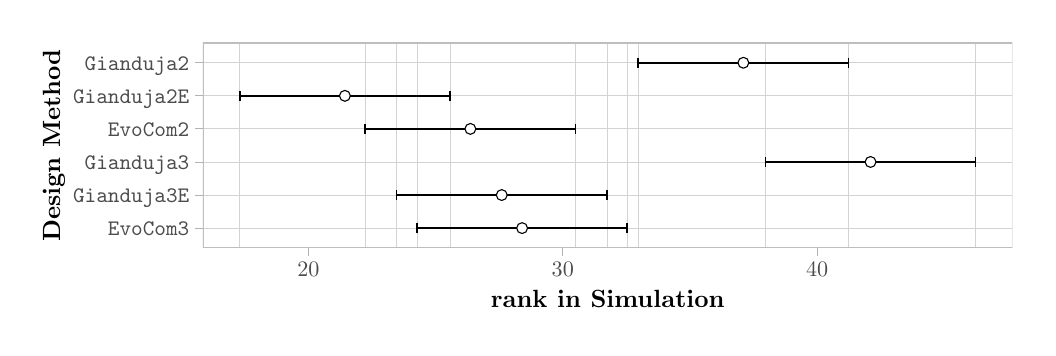
\begin{tikzpicture}[x=1pt,y=1pt]
\definecolor{fillColor}{RGB}{255,255,255}
\path[use as bounding box,fill=fillColor,fill opacity=0.00] (0,0) rectangle (361.35,108.41);
\begin{scope}
\path[clip] (  0.00,  0.00) rectangle (361.35,108.40);
\definecolor{drawColor}{RGB}{255,255,255}
\definecolor{fillColor}{RGB}{255,255,255}

\path[draw=drawColor,line width= 0.6pt,line join=round,line cap=round,fill=fillColor] (  0.00,  0.00) rectangle (361.35,108.40);
\end{scope}
\begin{scope}
\path[clip] ( 63.34, 28.81) rectangle (355.85,102.90);
\definecolor{fillColor}{RGB}{255,255,255}

\path[fill=fillColor] ( 63.34, 28.81) rectangle (355.85,102.90);
\definecolor{drawColor}{RGB}{211,211,211}

\path[draw=drawColor,line width= 0.3pt,line join=round] ( 63.34, 71.83) --
	(355.85, 71.83);

\path[draw=drawColor,line width= 0.3pt,line join=round] ( 63.34, 35.98) --
	(355.85, 35.98);

\path[draw=drawColor,line width= 0.3pt,line join=round] ( 63.34, 95.73) --
	(355.85, 95.73);

\path[draw=drawColor,line width= 0.3pt,line join=round] ( 63.34, 83.78) --
	(355.85, 83.78);

\path[draw=drawColor,line width= 0.3pt,line join=round] ( 63.34, 59.88) --
	(355.85, 59.88);

\path[draw=drawColor,line width= 0.3pt,line join=round] ( 63.34, 47.93) --
	(355.85, 47.93);

\path[draw=drawColor,line width= 0.2pt,line join=round] (197.95, 28.81) -- (197.95,102.90);

\path[draw=drawColor,line width= 0.2pt,line join=round] (296.60, 28.81) -- (296.60,102.90);

\path[draw=drawColor,line width= 0.2pt,line join=round] (152.61, 28.81) -- (152.61,102.90);

\path[draw=drawColor,line width= 0.2pt,line join=round] (216.64, 28.81) -- (216.64,102.90);

\path[draw=drawColor,line width= 0.2pt,line join=round] (342.55, 28.81) -- (342.55,102.90);

\path[draw=drawColor,line width= 0.2pt,line join=round] (209.29, 28.81) -- (209.29,102.90);

\path[draw=drawColor,line width= 0.2pt,line join=round] (121.98, 28.81) -- (121.98,102.90);

\path[draw=drawColor,line width= 0.2pt,line join=round] (220.63, 28.81) -- (220.63,102.90);

\path[draw=drawColor,line width= 0.2pt,line join=round] ( 76.64, 28.81) -- ( 76.64,102.90);

\path[draw=drawColor,line width= 0.2pt,line join=round] (140.67, 28.81) -- (140.67,102.90);

\path[draw=drawColor,line width= 0.2pt,line join=round] (266.58, 28.81) -- (266.58,102.90);

\path[draw=drawColor,line width= 0.2pt,line join=round] (133.32, 28.81) -- (133.32,102.90);
\definecolor{drawColor}{RGB}{0,0,0}

\path[draw=drawColor,line width= 0.6pt,line join=round] (197.95, 70.04) --
	(197.95, 73.62);

\path[draw=drawColor,line width= 0.6pt,line join=round] (197.95, 71.83) --
	(121.98, 71.83);

\path[draw=drawColor,line width= 0.6pt,line join=round] (121.98, 70.04) --
	(121.98, 73.62);

\path[draw=drawColor,line width= 0.6pt,line join=round] (296.60, 93.94) --
	(296.60, 97.53);

\path[draw=drawColor,line width= 0.6pt,line join=round] (296.60, 95.73) --
	(220.63, 95.73);

\path[draw=drawColor,line width= 0.6pt,line join=round] (220.63, 93.94) --
	(220.63, 97.53);

\path[draw=drawColor,line width= 0.6pt,line join=round] (152.61, 81.99) --
	(152.61, 85.58);

\path[draw=drawColor,line width= 0.6pt,line join=round] (152.61, 83.78) --
	( 76.64, 83.78);

\path[draw=drawColor,line width= 0.6pt,line join=round] ( 76.64, 81.99) --
	( 76.64, 85.58);

\path[draw=drawColor,line width= 0.6pt,line join=round] (216.64, 34.19) --
	(216.64, 37.77);

\path[draw=drawColor,line width= 0.6pt,line join=round] (216.64, 35.98) --
	(140.67, 35.98);

\path[draw=drawColor,line width= 0.6pt,line join=round] (140.67, 34.19) --
	(140.67, 37.77);

\path[draw=drawColor,line width= 0.6pt,line join=round] (342.55, 58.09) --
	(342.55, 61.67);

\path[draw=drawColor,line width= 0.6pt,line join=round] (342.55, 59.88) --
	(266.58, 59.88);

\path[draw=drawColor,line width= 0.6pt,line join=round] (266.58, 58.09) --
	(266.58, 61.67);

\path[draw=drawColor,line width= 0.6pt,line join=round] (209.29, 46.14) --
	(209.29, 49.72);

\path[draw=drawColor,line width= 0.6pt,line join=round] (209.29, 47.93) --
	(133.32, 47.93);

\path[draw=drawColor,line width= 0.6pt,line join=round] (133.32, 46.14) --
	(133.32, 49.72);

\path[draw=drawColor,line width= 0.4pt,line join=round,line cap=round,fill=fillColor] (159.97, 71.83) circle (  1.96);

\path[draw=drawColor,line width= 0.4pt,line join=round,line cap=round,fill=fillColor] (258.62, 95.73) circle (  1.96);

\path[draw=drawColor,line width= 0.4pt,line join=round,line cap=round,fill=fillColor] (114.63, 83.78) circle (  1.96);

\path[draw=drawColor,line width= 0.4pt,line join=round,line cap=round,fill=fillColor] (178.66, 35.98) circle (  1.96);

\path[draw=drawColor,line width= 0.4pt,line join=round,line cap=round,fill=fillColor] (304.57, 59.88) circle (  1.96);

\path[draw=drawColor,line width= 0.4pt,line join=round,line cap=round,fill=fillColor] (171.30, 47.93) circle (  1.96);
\definecolor{drawColor}{RGB}{190,190,190}

\path[draw=drawColor,line width= 0.6pt,line join=round,line cap=round] ( 63.34, 28.81) rectangle (355.85,102.90);
\end{scope}
\begin{scope}
\path[clip] (  0.00,  0.00) rectangle (361.35,108.41);
\definecolor{drawColor}{gray}{0.30}

\node[text=drawColor,anchor=base east,inner sep=0pt, outer sep=0pt, scale=  0.80] at ( 58.39, 69.08) {\texttt{EvoCom2}};

\node[text=drawColor,anchor=base east,inner sep=0pt, outer sep=0pt, scale=  0.80] at ( 58.39, 33.22) {\texttt{EvoCom3}};

\node[text=drawColor,anchor=base east,inner sep=0pt, outer sep=0pt, scale=  0.80] at ( 58.39, 92.98) {\texttt{Gianduja2}};

\node[text=drawColor,anchor=base east,inner sep=0pt, outer sep=0pt, scale=  0.80] at ( 58.39, 81.03) {\texttt{Gianduja2E}};

\node[text=drawColor,anchor=base east,inner sep=0pt, outer sep=0pt, scale=  0.80] at ( 58.39, 57.13) {\texttt{Gianduja3}};

\node[text=drawColor,anchor=base east,inner sep=0pt, outer sep=0pt, scale=  0.80] at ( 58.39, 45.18) {\texttt{Gianduja3E}};
\end{scope}
\begin{scope}
\path[clip] (  0.00,  0.00) rectangle (361.35,108.41);
\definecolor{drawColor}{gray}{0.70}

\path[draw=drawColor,line width= 0.3pt,line join=round] ( 60.59, 71.83) --
	( 63.34, 71.83);

\path[draw=drawColor,line width= 0.3pt,line join=round] ( 60.59, 35.98) --
	( 63.34, 35.98);

\path[draw=drawColor,line width= 0.3pt,line join=round] ( 60.59, 95.73) --
	( 63.34, 95.73);

\path[draw=drawColor,line width= 0.3pt,line join=round] ( 60.59, 83.78) --
	( 63.34, 83.78);

\path[draw=drawColor,line width= 0.3pt,line join=round] ( 60.59, 59.88) --
	( 63.34, 59.88);

\path[draw=drawColor,line width= 0.3pt,line join=round] ( 60.59, 47.93) --
	( 63.34, 47.93);
\end{scope}
\begin{scope}
\path[clip] (  0.00,  0.00) rectangle (361.35,108.41);
\definecolor{drawColor}{gray}{0.70}

\path[draw=drawColor,line width= 0.3pt,line join=round] (101.45, 26.06) --
	(101.45, 28.81);

\path[draw=drawColor,line width= 0.3pt,line join=round] (193.36, 26.06) --
	(193.36, 28.81);

\path[draw=drawColor,line width= 0.3pt,line join=round] (285.27, 26.06) --
	(285.27, 28.81);
\end{scope}
\begin{scope}
\path[clip] (  0.00,  0.00) rectangle (361.35,108.41);
\definecolor{drawColor}{gray}{0.30}

\node[text=drawColor,anchor=base,inner sep=0pt, outer sep=0pt, scale=  0.80] at (101.45, 18.35) {20};

\node[text=drawColor,anchor=base,inner sep=0pt, outer sep=0pt, scale=  0.80] at (193.36, 18.35) {30};

\node[text=drawColor,anchor=base,inner sep=0pt, outer sep=0pt, scale=  0.80] at (285.27, 18.35) {40};
\end{scope}
\begin{scope}
\path[clip] (  0.00,  0.00) rectangle (361.35,108.41);
\definecolor{drawColor}{RGB}{0,0,0}

\node[text=drawColor,anchor=base,inner sep=0pt, outer sep=0pt, scale=  0.90] at (209.60,  7.44) {\bfseries rank in Simulation};
\end{scope}
\begin{scope}
\path[clip] (  0.00,  0.00) rectangle (361.35,108.41);
\definecolor{drawColor}{RGB}{0,0,0}

\node[text=drawColor,rotate= 90.00,anchor=base,inner sep=0pt, outer sep=0pt, scale=  0.90] at ( 11.71, 65.86) {\bfseries Design Method};
\end{scope}
\end{tikzpicture}
